\chapter{Datanın Doğrulanması}
Olay üretimimizde çeşitli aralıktati $H_t$ lere göre üretim yapmış bulunmaktayız. Bu üretilen olaylar Tablo \ref{olay} da verilmiştir.
\begin{table}[!htpb]
\begin{tabular}{|c|c|c|c|c|}
\hline 
$H_t bin (GeV)$ & $Event_{nonmatch}$ & $\sigma_{nonmatch}$ & $Event_{match}$ & $\sigma_{match}$ \\ 
\hline 
100-250 & 500000 & $3.48 \times 10^7$ & 234162 & $1.634 \times 10^7$ \\ 
\hline 
250-500 & 500000 & $2.487 \times 10^6$ & 121332 & $6.065 \times 10^4$ \\ 
\hline 
500-1000 & 500000 & $1.827 \times 10^5$ & 85325 & $3.098 \times 10^4$ \\ 
\hline 
1000-2500 & 500000 & 8101 & 65388 & 1070 \\ 
\hline 
2500-4000 & 500000 & $37.64$ & 53737 & 4.048 \\ 
\hline 
4000-6000 & 500000 & 0.8119 & 53212 & 0.08667 \\ 
\hline 
6000-$\inf$ & 500000 & $0.00721 \times 10^{-6}$ & 58455 & 0.0008565 \\ 
\hline 
\end{tabular} 
\label{olay}
\caption{Üretilen olaylar}
\end{table}
Bir olayda toplam $H_t$ hesabı için;
\begin{equation}
H_t = \sum_{i=1}^N p_{T_i}
\end{equation}
formülünü kullanmaktayız. 

\par Yukarıda tabloda verilen olayların üzerinde analiz yapmak için bu üretilen dosyaların hepsini birleştirmemiz gerekir. Bu birleştirme işlemi için 2 yol mevcut. 1. yol \textbf{root} programının kodu olan \textbf{hadd} ile birleştirmek. Bu kodun kullanımı terminal üzerinden;
\begin{lstlisting}
hadd target.root source1.root source2.root ... sourceN.root
\end{lstlisting}
şeklinde yapılmaktadır. Bu birleştirme işlemi gerçekleştirilirken birleştirilecek olan grafikteki değerler herhangi bir ağırlıklandırılma yapılmadan birleştiriliyor. Şekil \ref{fig:hadd} de görüldüğü gibi sağ taraftaki grafikle peakler mevcut ve analizimiz doğru sonuç vermeyecek. Çünkü üretilen olayların olay sayıları ve saçılma tesir kesitleri farklı ve herbiri toplam olaya farklı katkıda bulunacak. Bunun için elde ettiğimiz ayrı ayrı verileri ağırlandırarak birleştirdik. Böylece ürettiğimiz her data parçası toplam olaya aynı katkıda bulundu. Ağırlıklandırma yaparak birleştirme işleminde \textbf{C} programla diliyle;
\begin{lstlisting}
.
.
.
void MergeRootfile( TDirectory *target, TList *sourcelist, double crossArray[] );
// List of Cross-sections divided by num of events produced
double crossSections[7] = {
      16340000.0/234162.,
      606500.0/121332.,
      30980.0/85325.,
      1070.0/65388.,
      4.048/53737.,
      0.08667/53212.,
      0.0008565/58455.};
void hadd(){
   // in an interactive ROOT session, edit the file names
   // Target and FileList, then
   // root > .L hadd.C
   // root > hadd()
  Target = TFile::Open( "result_last.root", "RECREATE" );
  FileList = new TList();
  // ************************************************************
  // List of Files
  FileList->Add( TFile::Open("analysis_100-250.root") );  // 3
  FileList->Add( TFile::Open("analysis_250-500.root") );  // 4
  FileList->Add( TFile::Open("analysis_500-1000.root") );  // 5
  FileList->Add( TFile::Open("analysis_1000-2500.root") ); // 6
  FileList->Add( TFile::Open("analysis_2500-4000.root") );// 7
  FileList->Add( TFile::Open("analysis_4000-6000.root") );// 8
  FileList->Add( TFile::Open("analysis_6000-Inf.root") );// 9
  // ************************************************************
  MergeRootfile( Target, FileList, crossSections );
}
.
.
.
\end{lstlisting}
şeklinde birleştirme işlemini gerçekleştirdik.
\par Ürettiğimiz olayların içinden sadece bazı olayları aldık. Bu olayları seçerken, bir olaydan 2 veya daha fazla Jet çıkması, $H_t > 0.2 TeV$ ,$p_T > 50 GeV$ ve son olarak $|y|< 2.5$ koşuluna uyan olayları alıp bunun üzerinden analizimizi yaptık.
\begin{figure}[!htpb]
\centering
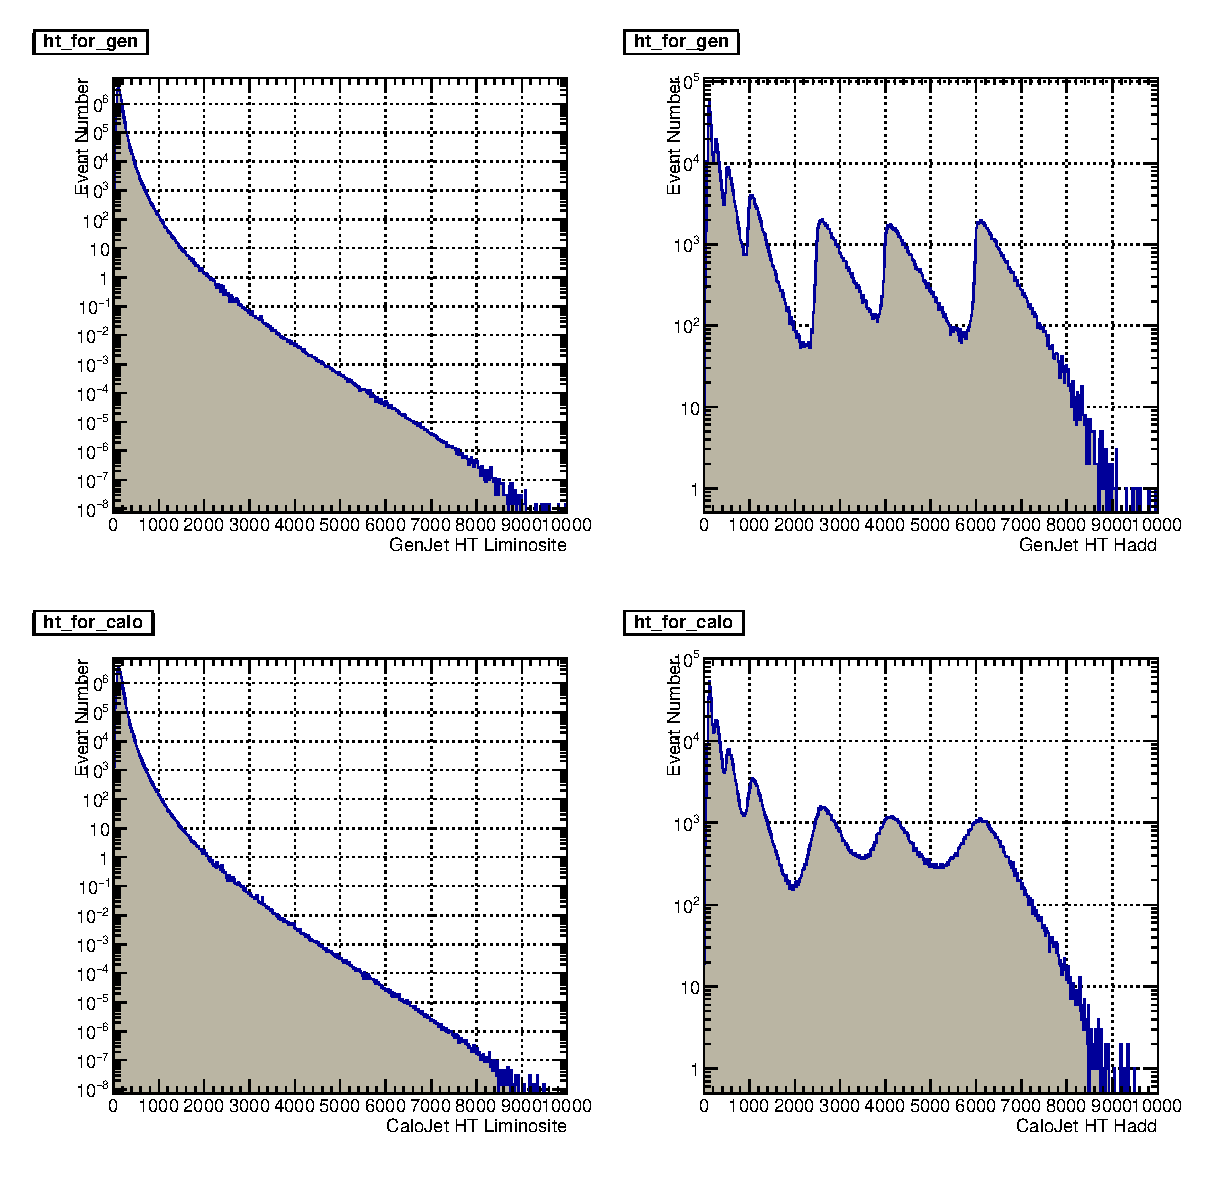
\includegraphics[scale=0.8]{jet_ht.eps}
\caption{Sol tarafta ağırlıklandırma yapılarak birleştirilmiş GenJet $p_T$ leri ve CaloJet $p_T$ leri. Sağ tarafta \textbf{hadd} kullanımı sonucu}
\label{fig:hadd}
\end{figure}

\begin{figure}[!htpb] 
\centering
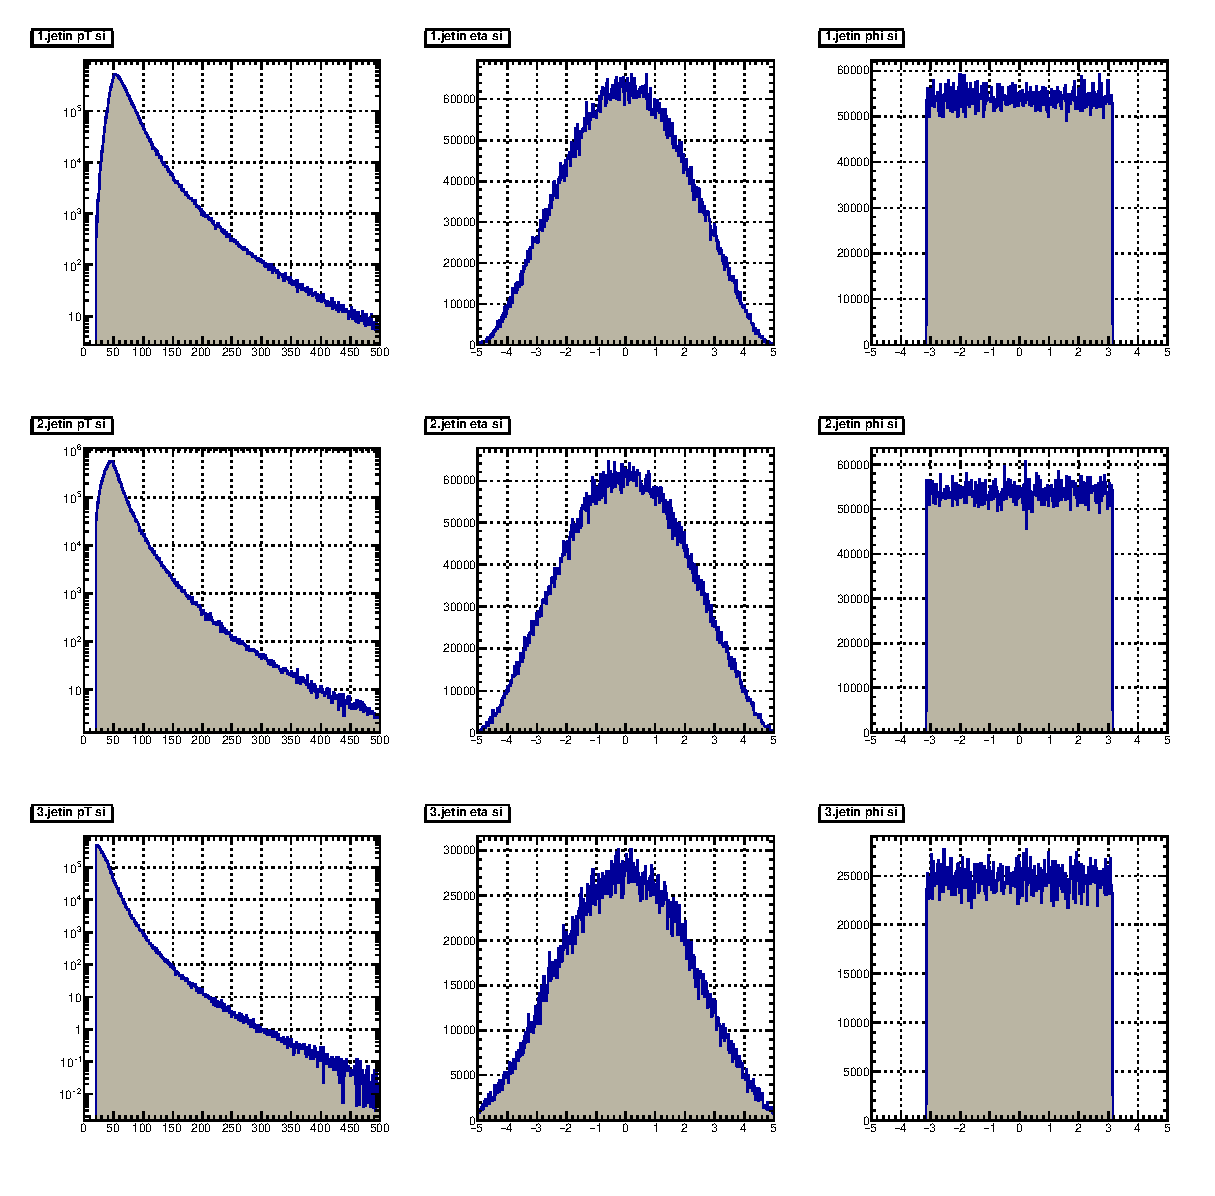
\includegraphics[scale=0.8]{pt_eta_phi.eps}
\caption{İlk üç Jetin $p_T$ $\eta$ ve $\phi$ dağılımları}
\label{fig:ptetaphi}
\end{figure}
\par Şekil \ref{fig:ptetaphi} ilk satırda en yüksek $p_T$ ye sahip olan ikinci satırdaki ikinci en yüksek ve son olrak üçüncü en yüksek $p_T$ ye sahip olan Jetlerin enerji dağılımları ve dedektör sistemine göre ta
\begin{figure}[!htpb] 
\centering
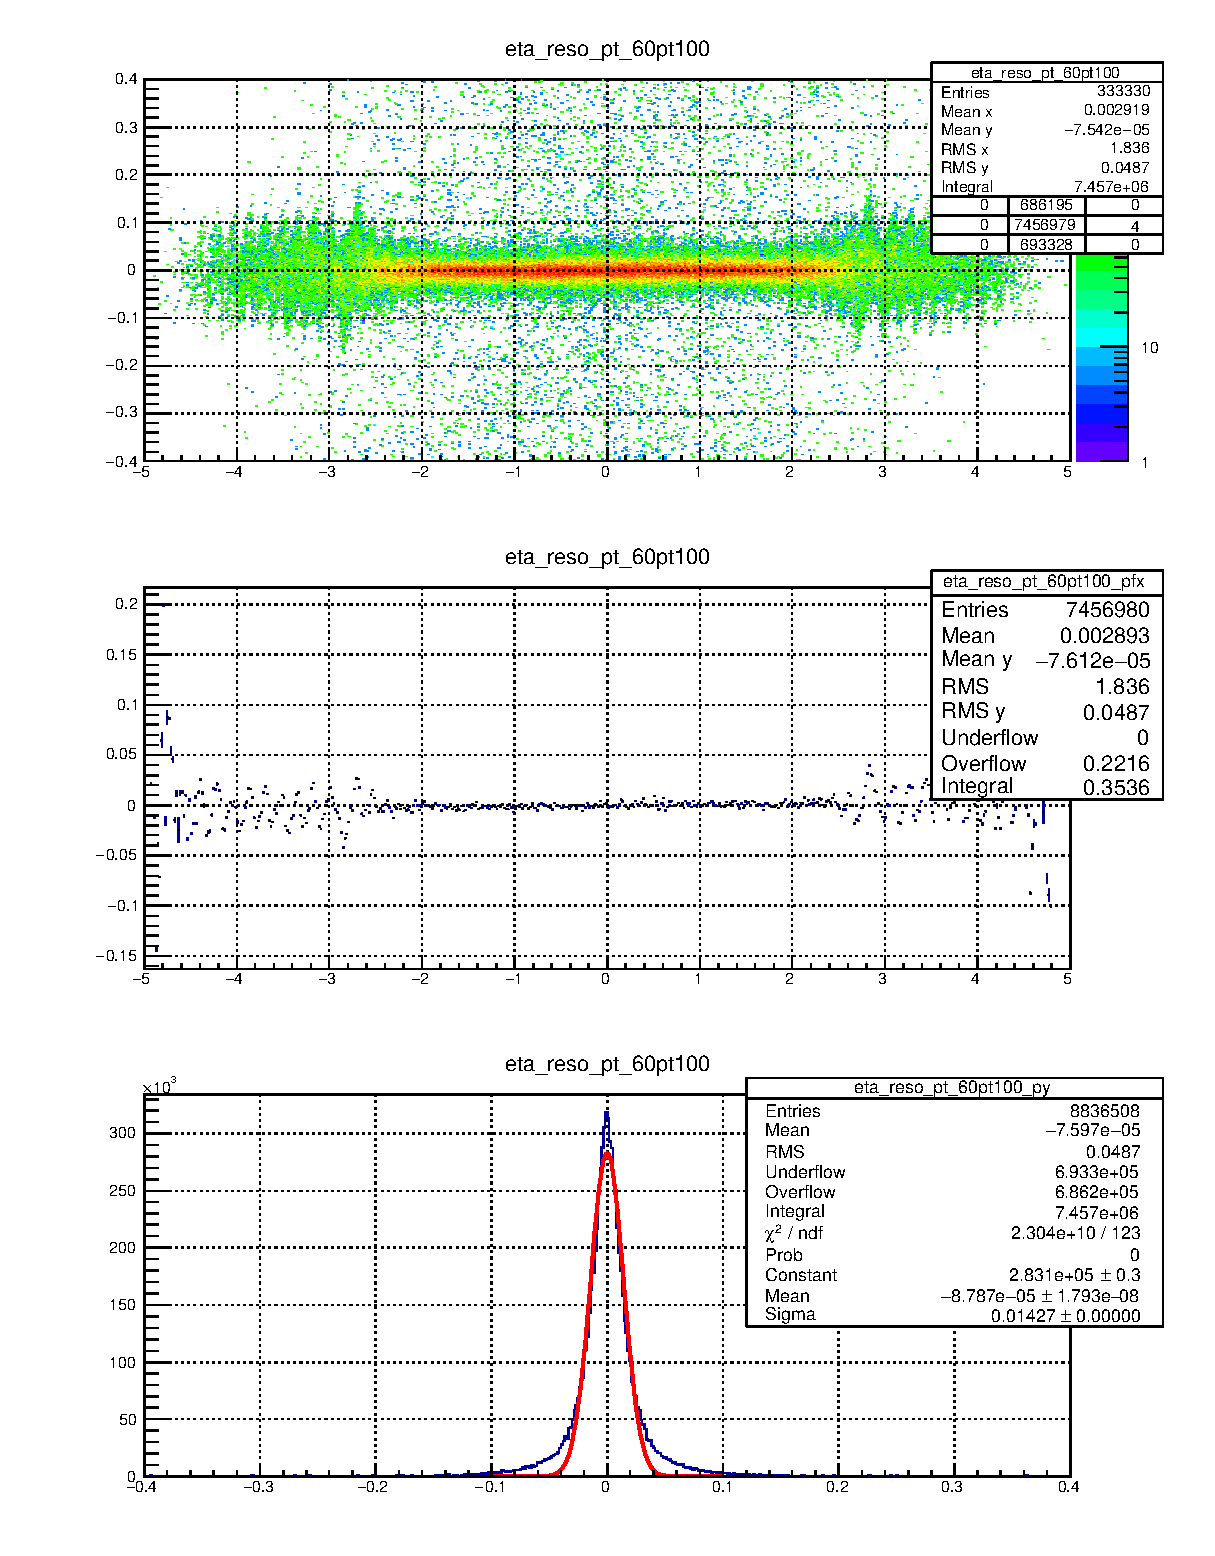
\includegraphics[scale=0.25]{eta_reso_pt_60pt100.eps}
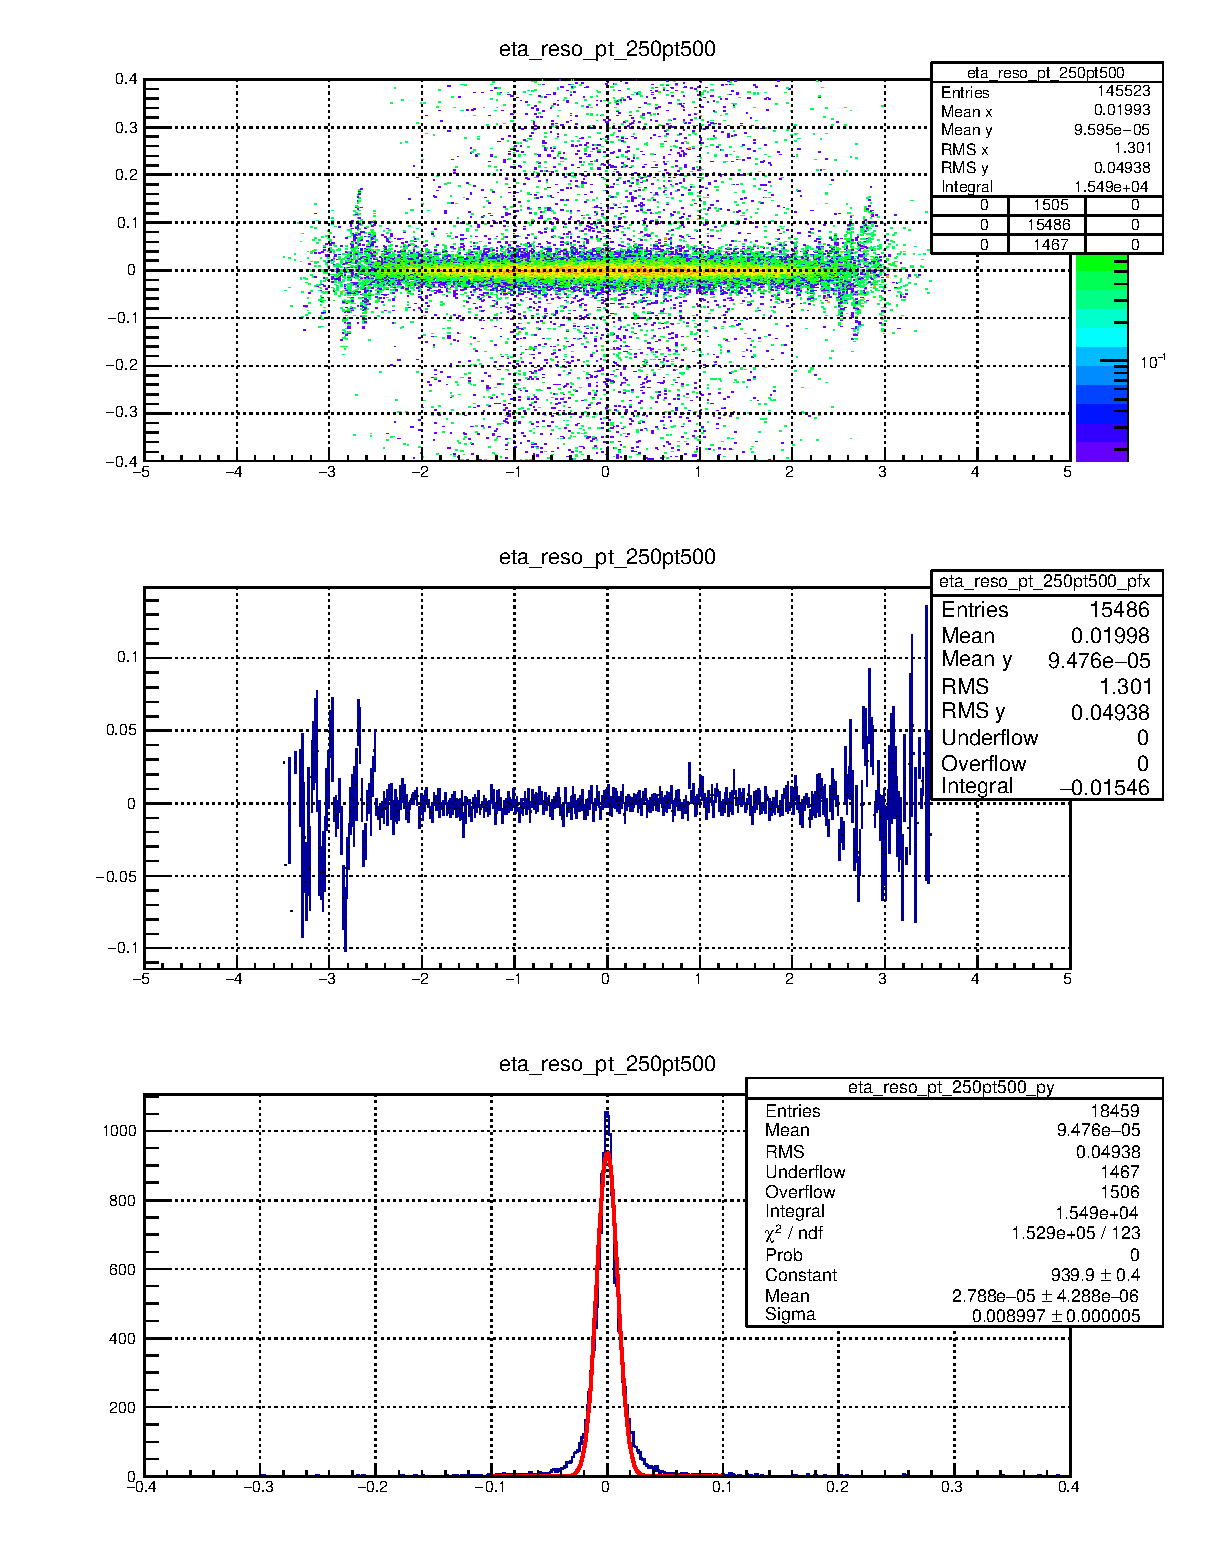
\includegraphics[scale=0.25]{eta_reso_pt_250pt500.eps}
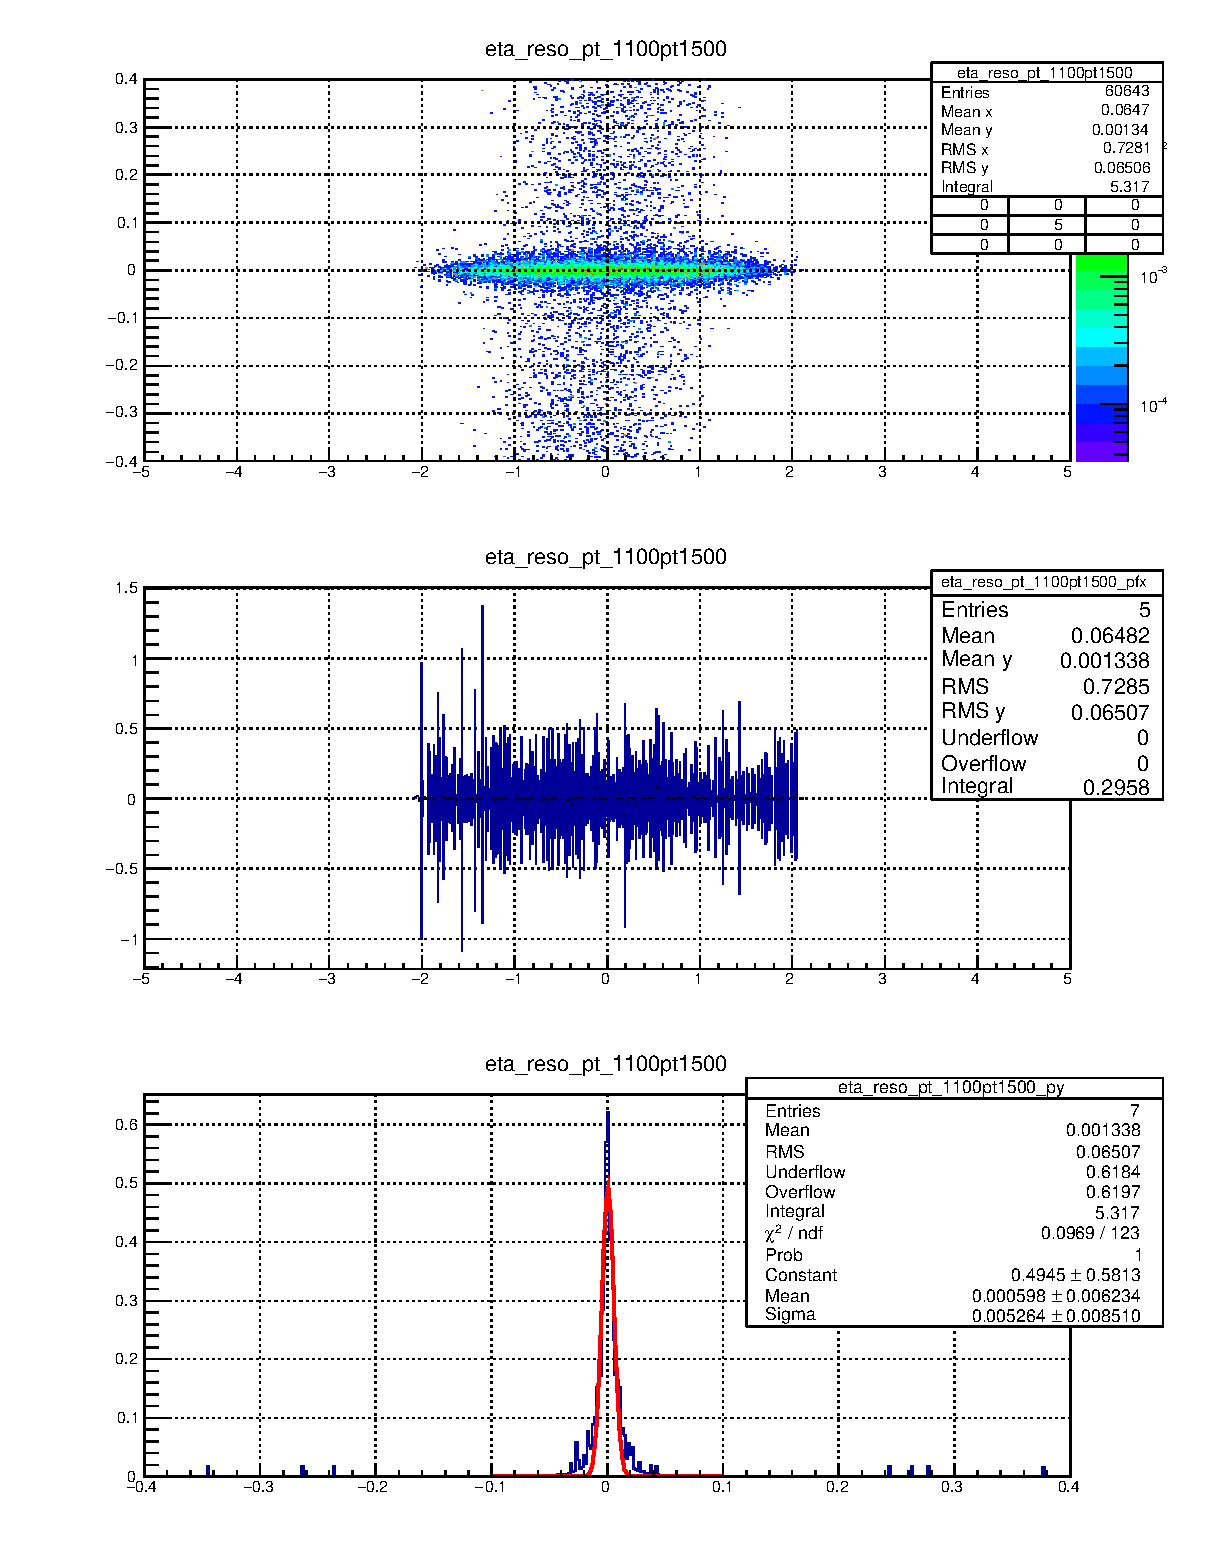
\includegraphics[scale=0.25]{eta_reso_pt_1100pt1500.eps}
\caption{farklı pt aralıkları için eta resolution}
\end{figure}


